% ============================================================
% Background and Related Work — draft v1
% All citation keys resolve against references.bib (v. 2026-10-16b).
% Figures reused from the previous draft: figures/tile_concept_overview.png,
% figures/pyramid_generalization.png. New TikZ figure: fig_mvt_mlt_streams.tex.
% Requires: natbib, graphicx, tikz.
% ============================================================

\section{Background and Related Work}
\label{sec:background}

This section introduces the concepts the study relies on: how tiled vector maps are
organized (Section~\ref{sec:bg-tiling}), how practitioners already depart from the
conventional tile pyramid (Section~\ref{sec:bg-overzoom}), how MVT and MLT lay out the
content of a tile (Section~\ref{sec:bg-encodings}), and why the size of an
independently encoded unit matters for compression (Section~\ref{sec:bg-granularity}).
Section~\ref{sec:bg-related} positions the study with respect to prior work.

% ------------------------------------------------------------
\subsection{Tiled vector maps}
\label{sec:bg-tiling}

Web maps are not delivered as a single file. The world is divided into square tiles at
a series of zoom levels, and a client downloads only the tiles that cover its current
view \citep{osm_slippy_tiles}; with vector tiles the client also styles and draws their
content itself. At zoom~0 a single tile covers the world, and each level
splits every tile into four, so a complete level~$z$ contains $4^z$ tiles. A tile is
addressed by its zoom, column and row, written $z/x/y$, and archives such as PMTiles map
each address to a stored tile \citep{pmtiles_v3}. More general tiling schemes, with other
projections and tile matrices, are standardized by the OGC Two Dimensional Tile Matrix
Set \citep{ogc2022tms}, but the quadtree scheme above is the one used by almost all web
vector maps. Figure~\ref{fig:tile-concept-overview} summarizes these concepts.

\begin{figure}[!tbp]
    \centering
    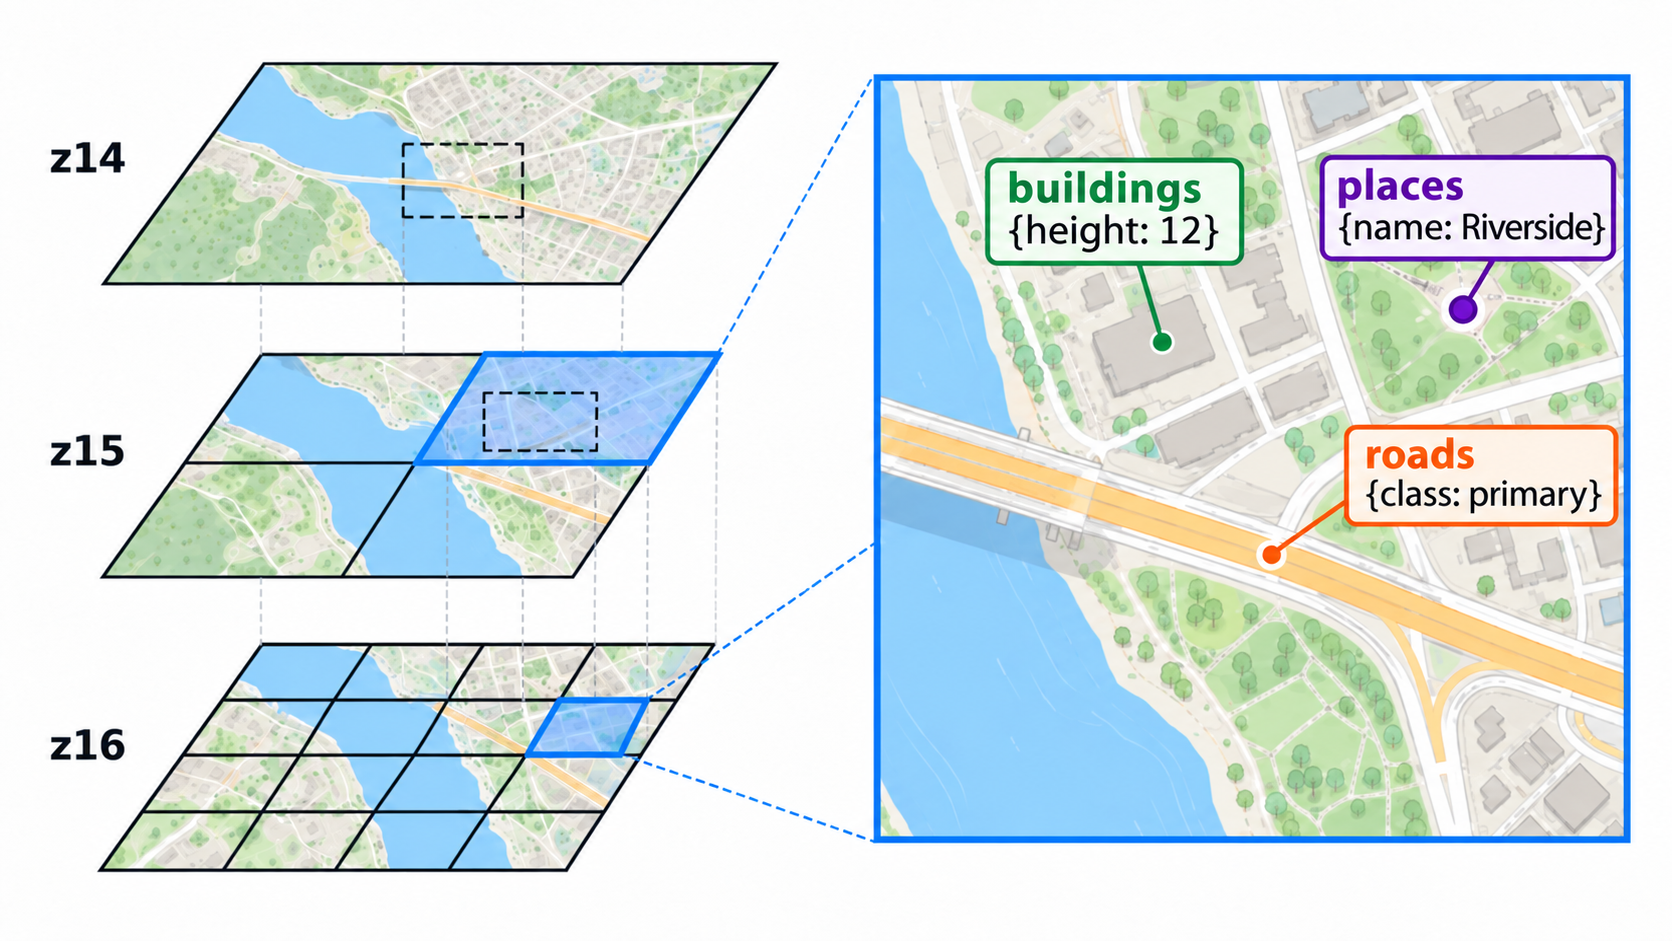
\includegraphics[width=\columnwidth]{figures/tile_concept_overview.png}
    \caption{A tile pyramid, parent and child tiles, a viewport, and the layers,
    coordinates, features and attributes stored in one tile.}
    \label{fig:tile-concept-overview}
\end{figure}

Each zoom level is generated for its own scale. At low zoom levels only major features
are kept and their shapes are simplified, while deeper levels add smaller features and
finer detail (Figure~\ref{fig:pyramid-generalization}). A tile is therefore a summary of
its area at one scale rather than the union of its four children. Production tile
generators also bound the size of each tile: Tippecanoe, for example, by default limits
a tile to 500~kB of compressed data and 200{,}000 features, lowers the resolution of
tiles that exceed the size limit, and offers options to drop or coalesce features
\citep{tippecanoe}.

\begin{figure}[!tbp]
    \centering
    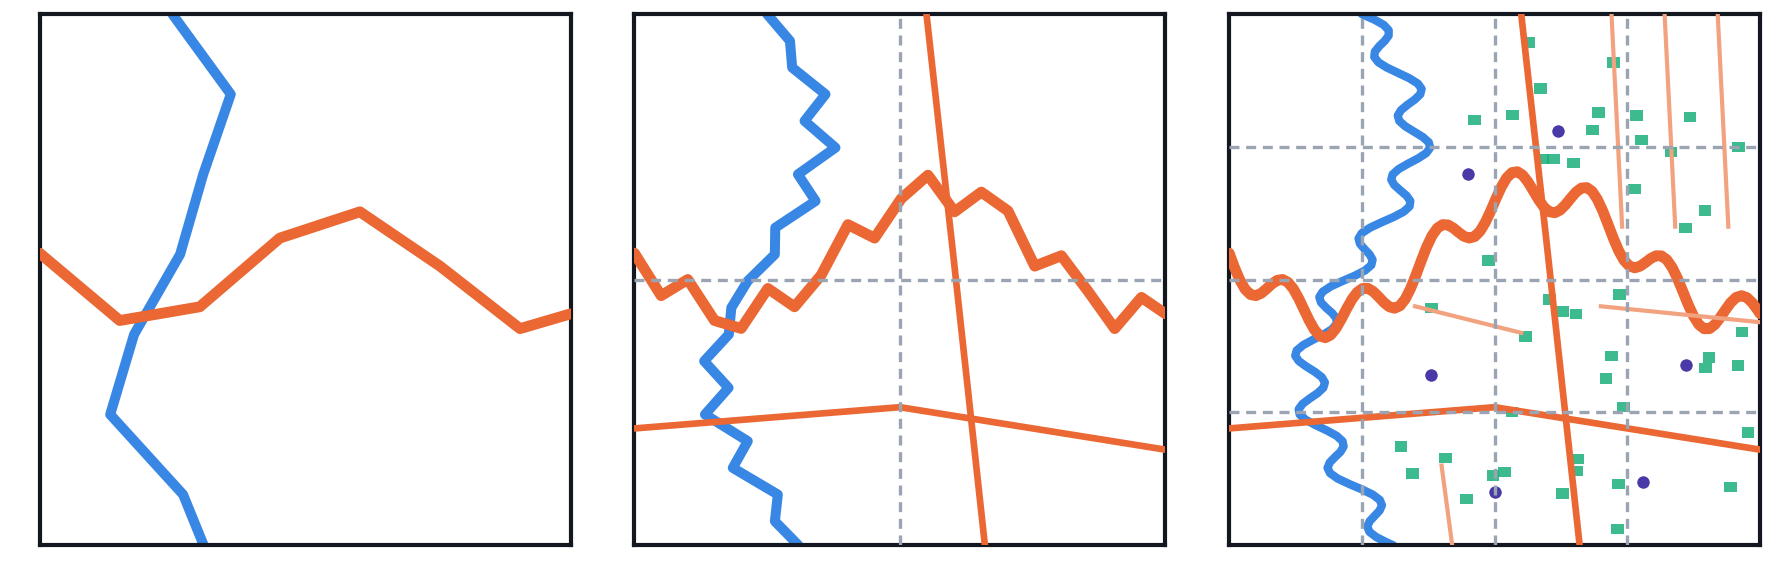
\includegraphics[width=\columnwidth]{figures/pyramid_generalization.png}
    \caption{The same area at three zoom levels: features and detail are added as
    zoom increases.}
    \label{fig:pyramid-generalization}
\end{figure}

Inside a tile, geometry is stored as integer coordinates on a local grid, the
\emph{extent}, conventionally 4096$\times$4096 units \citep{mapbox_mvt_spec_2_1}.
The tile does not record its own position: its $z/x/y$ address is kept outside the tile,
and the tile format itself does not prescribe a pyramid \citep{mapbox_mvt_spec_2_1,
maplibre_mlt_overview}. Every tile is encoded independently, so an encoder can exploit
repetition only among the features of one tile, and each tile repeats its own layer,
column or stream structure.

We distinguish four quantities that are easily conflated. \emph{Spatial tile
granularity} is the geographic area and corresponding content grouped into one
independently encoded tile at a given logical level of detail. \emph{Coordinate extent}
is the integer grid used to represent coordinates inside that tile. \emph{Encoded tile
size} is the resulting number of bytes. \emph{Rendered tile size} is the screen-space
size used by a client. Increasing coordinate extent alone changes precision, not spatial
granularity; in our experiment it is increased together with spatial aggregation so that
the coarser encoding unit retains approximately the same coordinate precision.

% ------------------------------------------------------------
\subsection{Overzoom, metatiles and sparse pyramids}
\label{sec:bg-overzoom}

The dense quadtree pyramid is the default, but practitioners already depart from it,
mainly to reduce the number of stored tiles and requests.

\paragraph{Overzoom.} A client may display a tile at zoom levels deeper than the deepest
level stored, scaling the tile up instead of requesting its children. The extent is the
main limit on this practice: the extent field of MVT is an unsigned 32-bit integer whose
value 4096 is a default rather than a maximum \citep{mapbox_mvt_spec_2_1}, and MLT
declares the extent per layer and notes that a larger extent gives more precision at the
cost of more bytes \citep{maplibre_mlt_overview}. Developer proposals build on this.
A MapLibre proposal argued that ``using a large tile extent allows you to tile your
dataset only as far as is necessary'' \citep{maplibre_gljs_2507}; a Planetiler feature
request asks for an extent of 16384 at the maximum zoom so that a small tileset can be
overzoomed, instead of raising the maximum zoom, which would greatly increase the archive
size \citep{planetiler_1286}; and Tippecanoe can add extra detail at the maximum zoom to
improve precision when overzooming \citep{tippecanoe}. On the client side, MapLibre GL JS
now splits a deep-overzoomed source tile into virtual child tiles in a worker and
overscales only the last few levels, by default four \citep{maplibre_gljs_mapoptions}.

\paragraph{Metatiles.} Raster tile servers commonly render and store \emph{metatiles},
usually blocks of $8\times8$ tiles, because rendering one large area is cheaper than
rendering many small ones, labels are placed more consistently, and fewer files need to
be stored \citep{osm_wiki_metatiles}. Metatiles are a server-side unit, however: clients
still request and receive individual tiles.

\paragraph{Larger tiles.} Vector tile services have also offered larger tiles directly.
The Tilezen service (formerly Mapzen) served 256- and 512-pixel tiles, stating that
a single 512-pixel request is equivalent to four 256-pixel requests, and listed fewer
requests, better label placement, smaller files and less disk space for offline use
among the advantages of the larger size \citep{tilezen_service}. The 512-pixel vector
tile has since become the convention of WebGL renderers such as MapLibre GL JS
\citep{maplibre_gljs_vectorsource}.

\paragraph{Sparse pyramids.} Tippecanoe can generate a variable-depth pyramid that omits
child tiles wherever the parent is detailed enough to be overzoomed \citep{tippecanoe}.
A corresponding Planetiler proposal asks for variable tile depth so that descendants
need not be generated where an ancestor already represents the required detail
\citep{planetiler_1574}. Archives such as PMTiles can store such sparse pyramids, but
clients need a way to distinguish a tile that is intentionally missing, and should be
replaced by an overzoomed ancestor, from one that is empty. A design proposal for
MapLibre adds this distinction to tiled sources and TileJSON
\citep{maplibre_stylespec_1869}.

\paragraph{The rendered tile.} These approaches increase how much information a stored
tile carries, but not the size of the unit that the client renders: MapLibre GL JS, for
example, requires vector sources to use a tile size of 512 pixels
\citep{maplibre_gljs_vectorsource}. Their motivations are primarily rendering precision,
storage and request count. They do not provide a controlled measurement of compression
as a function of the spatial boundary of one independently encoded unit. The denser
variants studied here apply a related idea at every logical zoom: a tile covers the area
of multiple conventional cells while a larger coordinate extent preserves approximately
the same spatial precision.

% ------------------------------------------------------------
\subsection{Feature-oriented and column-oriented tile encodings}
\label{sec:bg-encodings}

The Mapbox Vector Tile (MVT) format encodes a tile as a Protocol Buffers message with
named layers. Each layer holds a sequence of feature records; a record contains the
feature's geometry, written as integer drawing commands with zigzag-encoded coordinate
deltas, and its attributes, written as indices into tables of keys and values shared by
the layer \citep{mapbox_mvt_spec_2_1}. The layout is thus feature-oriented
(Figure~\ref{fig:mvt-mlt-streams}a), and redundancy across features is exploited mainly
through the shared key and value tables and, in practice, by gzip applied to the whole
tile.

MapLibre Tiles (MLT) organizes vector-tile content by column
\citep{tremmel2025mlt, maplibre_mlt_v1}. Within a layer, each property of all features,
such as geometry type, vertex offsets, vertex coordinates or an attribute, is stored as
a column, and each column is split into \emph{streams} of same-typed values, for example
presence, data, length and offset streams. Every stream carries its own metadata,
namely the number of values, the byte length and the encoding
\citep{maplibre_mlt_overview}. Streams are compressed with lightweight encodings such as
dictionary, run-length and delta encoding combined with integer packing, chosen per
stream by the encoder (Figure~\ref{fig:mvt-mlt-streams}b). The original evaluation reports
compression up to three times better than MVT over whole tilesets and more than six
times better for some large tiles \citep{tremmel2025mlt}. MapLibre's public benchmarks on
two planet-scale basemaps report smaller gains after gzip: the stable MLT~v1 reduces
gzipped archive size by about 15\% for OpenMapTiles and 5\% for Protomaps, and the
experimental MLT~v2 by about 18\% and 10\% \citep{maplibre_mlt_benchmarks}.
The same benchmarks show that disabling a dictionary shared by several columns enlarges
the uncompressed archive by about 25\% for one of the two basemaps \citep{maplibre_mlt_benchmarks},
an indication of how much the format depends on redundancy that exists within one tile.
Unlike MVT's per-feature property types, MLT declares one type per property column
within a layer of a tile; mixed input types therefore require normalization during
conversion \citep{maplibre_mlt_mvt_compat}.


The pinned Rust implementation also supports experimental MLT v2. It retains the
columnar layer model while changing stream/schema metadata, interleaved integer RLE
and FastPFOR block layout, and supporting bit-packed dictionary codes. Additional
v2 codecs exist but are disabled in this experiment. We compare versions with the
same common settings as a robustness test, not as a codec-option benchmark
\citep{maplibre_mlt_rust_pinned}.

% Figure: feature-oriented (MVT) vs column-oriented (MLT) layout of one layer,
% and the effect of encoding-unit size on fixed per-stream metadata.
% Requires: \usepackage{tikz}
\begin{figure*}[t]
\centering
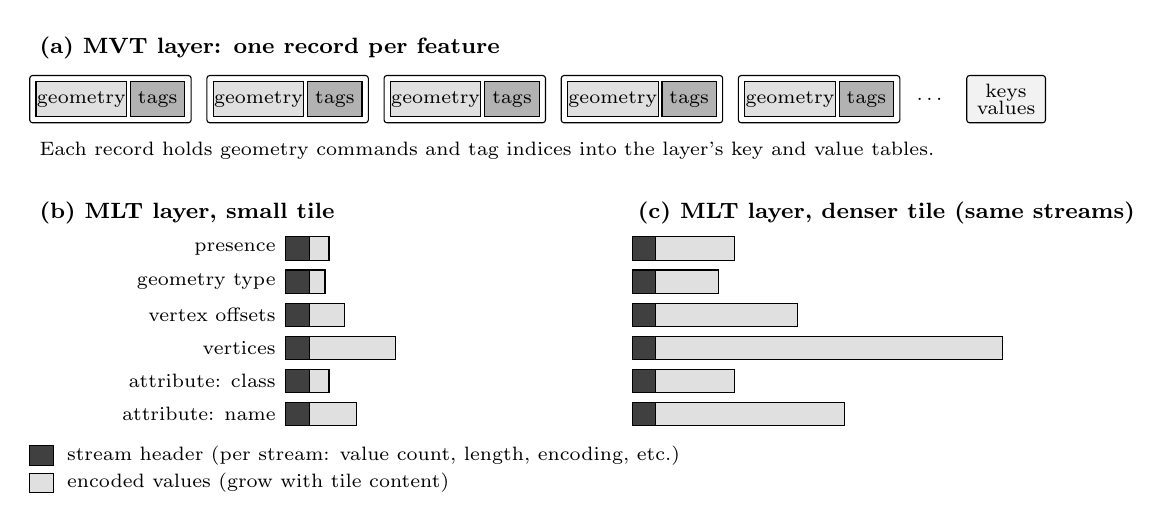
\begin{tikzpicture}[x=1cm, y=1cm, font=\scriptsize,
    hdr/.style={draw, fill=black!75, minimum height=0.32cm, inner sep=0pt},
    pay/.style={draw, fill=black!12},
    rec/.style={draw, rounded corners=1pt},
    lbl/.style={anchor=east, inner sep=2pt}]

  % ---------------- (a) MVT ----------------
  \node[anchor=west, font=\footnotesize\bfseries] at (-2.6,3.55)
        {(a) MVT layer: one record per feature};
  \foreach \i in {0,...,4} {
    \pgfmathsetmacro{\x}{-2.6+\i*2.25}
    \draw[rec] (\x,2.6) rectangle ++(2.05,0.6);
    \draw[pay] (\x+0.08,2.68) rectangle ++(1.15,0.44);
    \node at (\x+0.655,2.9) {geometry};
    \draw[draw, fill=black!30] (\x+1.28,2.68) rectangle ++(0.69,0.44);
    \node at (\x+1.625,2.9) {tags};
  }
  \node at (8.85,2.9) {\dots};
  \draw[rec, fill=black!5] (9.3,2.6) rectangle ++(1.0,0.6);
  \node[align=center] at (9.8,2.9) {keys\\[-2pt]values};
  \node[anchor=west] at (-2.6,2.25)
        {Each record holds geometry commands and tag indices into the layer's key and value tables.};

  % ---------------- (b) MLT, small tile ----------------
  \node[anchor=west, font=\footnotesize\bfseries] at (-2.6,1.45)
        {(b) MLT layer, small tile};
  \node[anchor=west, font=\footnotesize\bfseries] at (5.0,1.45)
        {(c) MLT layer, denser tile (same streams)};

  \def\names{{"presence","geometry type","vertex offsets","vertices","attribute: class","attribute: name"}}
  \def\small{{0.25,0.20,0.45,1.10,0.25,0.60}}
  \foreach \k in {0,...,5} {
    \pgfmathsetmacro{\y}{1.0-\k*0.42}
    \pgfmathparse{\names[\k]}\edef\nm{\pgfmathresult}
    \pgfmathsetmacro{\w}{\small[\k]}
    \pgfmathsetmacro{\W}{min(4*\small[\k],4.6)}
    % small tile
    \node[lbl] at (0.6,\y) {\nm};
    \draw[fill=black!75] (0.65,\y-0.15) rectangle ++(0.3,0.30);
    \draw[pay] (0.95,\y-0.15) rectangle ++(\w,0.30);
    % dense tile
    \draw[fill=black!75] (5.05,\y-0.15) rectangle ++(0.3,0.30);
    \draw[pay] (5.35,\y-0.15) rectangle ++(\W,0.30);
  }

  % legend
  \draw[fill=black!75] (-2.6,-1.75) rectangle ++(0.3,0.25);
  \node[anchor=west] at (-2.25,-1.625) {stream header (per stream: value count, length, encoding, etc.)};
  \draw[pay] (-2.6,-2.1) rectangle ++(0.3,0.25);
  \node[anchor=west] at (-2.25,-1.975) {encoded values (grow with tile content)};
\end{tikzpicture}
\caption{Feature-oriented and column-oriented layouts of one tile layer.
(a)~MVT stores a sequence of feature records.
(b)~MLT stores each property of all features as a column, split into streams of same-typed values;
every stream carries a header.
(c)~When a spatial encoding unit holds more content, streams become longer, amortizing per-stream
headers and exposing longer value sequences to lightweight encodings. MLT also contains layer- and
column-level structural bytes not drawn here; Section~\ref{sec:results-streams} reports total
non-payload structural share separately from stream-header share. Proportions are schematic.}
\label{fig:mvt-mlt-streams}
\end{figure*}

% ------------------------------------------------------------
\subsection{Encoding granularity in columnar storage and block compression}
\label{sec:bg-granularity}

The dependence of compression on the amount of data in one encoding unit is well known
outside cartography. Column stores compress data well because values of one column are
stored together and lightweight encodings can be applied to long runs of similar values
\citep{abadi2006compression}, and empirical studies of Parquet and ORC show that the
choice and effectiveness of encodings depend on the data within each unit
\citep{zeng2023columnar, kuschewski2023btrblocks}. These formats expose the unit size as a
parameter. Parquet lets the writer choose the size of row groups and data pages; its
documentation notes that larger pages carry less header overhead and recommends row
groups of 512~MB to 1~GB \citep{parquet_configurations}. ORC divides files into stripes of
typically about 200~MB and compresses streams in chunks of 256~kB by default, noting that
larger chunks compress better at the cost of memory \citep{orc_spec_v1}. Spatial Parquet
carries these ideas over to geospatial data lakes \citep{saeedan2022spatialparquet}.

General-purpose compressors show the same dependence. DEFLATE, the algorithm behind gzip,
finds repetitions within a sliding window of 32~kB \citep{rfc1951, rfc1952}, so data that
repeat across separately compressed files cannot be exploited. The Zstandard
documentation describes this as the small-data problem: the smaller the input, the
harder it is to compress, because at the start of a new input there is no past to build
upon, and it offers trained dictionaries, whose gains are concentrated in the first few
kilobytes, as a remedy \citep{zstd_readme}.

A vector tile differs from these settings in two ways. Its encoding unit is small,
typically kilobytes rather than megabytes (Appendix~\ref{app:traffic}), and its spatial
granularity is not a free parameter of the encoder: it follows from the tile matrix and
the generalization policy. Coordinate extent can be configured independently, but it
controls the local coordinate grid rather than the geographic area of the encoded unit.

% ------------------------------------------------------------
\subsection{Related work}
\label{sec:bg-related}

Prior work approaches this question from several adjacent directions. The original MLT
evaluation compares MLT and MVT on existing tiles and reports especially large gains for
some large tiles \citep{tremmel2025mlt}. MapLibre's current planet-scale benchmarks go
further and explicitly show that naturally large tiles benefit more from MLT
\citep{maplibre_mlt_benchmarks}. These are important precedents, but tile size is an
observed property of the corpus: the spatial boundary of the independently encoded tile
is not manipulated.

Other studies manipulate quantities that are related to granularity but confound it
with another change. GeoTile reports compressed vector-tile sizes across zoom levels,
where spatial footprint changes together with feature selection and level of detail
\citep{li2018geotile}. Feathered Tiles studies adaptive spatial partitioning and targets
roughly uniform tile payloads, but does not measure a compression-versus-partition-size
curve \citep{dufilie2014feathered}. HiFIVE systematically reduces byte size by pruning
records, attributes and values within a fixed tile, so its intervention is content
reduction rather than a change of the spatial encoding unit
\citep{bahadori2026hifive}. Variable-depth pyramids and overzooming in Tippecanoe and
Planetiler change which pyramid levels are stored, not the compression boundary at a
fixed logical zoom \citep{tippecanoe, planetiler_1574, planetiler_1286}.

These distinctions matter because changing zoom, fidelity, pyramid depth or observed
payload size does not isolate spatial granularity. To our knowledge, no prior work has
systematically varied the area represented by each independently encoded vector tile
under approximately matched-content and matched-LoD conditions and quantified the
resulting raw and externally compressed size, particularly for column-oriented MLT
relative to feature-oriented MVT. Studies of columnar storage
\citep{abadi2006compression, zeng2023columnar, kuschewski2023btrblocks,
saeedan2022spatialparquet} establish the general importance of encoding-unit size, but
at much larger, non-cartographic block sizes.
